\chapter{Strojno odvajanje}

V prejšnjem poglavju smo videli, da nam pri odvajanju funkcij koristi, 
če jih zapišemo v obliki računskega grafa in se nato pri odvajanju 
po grafu sprehodimo od konca proti začetku. Ta vzvratni »sprehod« 
(angl.\ \emph{back-propagation}) ustreza verižnemu pravilu odvajanja, 
pri čemer si vse vmesne rezultate zapomnimo in jih izračunamo natanko enkrat.

\marginnote{Pri razvoju postopka in kode za strojno odvajanje smo se močno zgledovali po izjemnem predavanju Andreja Karpathyja \emph{The spelled-out intro to neural networks and backpropagation: building micrograd}.}
Na osnovi tega vzvratnega sprehoda bomo zgradili algoritem oziroma 
implementirali kodo za strojno odvajanje. Pričeli bomo pri njegovem 
okostju~-- računskem grafu. Najprej bomo implementirali vozlišče grafa, 
mu dodali podatke o njegovih predhodnikih ter preverili, ali lahko 
računski graf uporabimo za izračun funkcijskih vrednosti 
(angl.\ \emph{forward computation}). Ko bomo s tem zadovoljni, 
bomo implementirali še izračun gradientov. Postopek bomo razvijali 
postopoma in ga zaključili z demonstracijo uporabnosti.

\section{Vozlišča v računskem grafu}

Čas je, da za strojno odvajanje spišemo tudi kodo, in sicer v programskem
jeziku Python. Začnimo s predstavitvijo vozlišča v računskem grafu, ki ga
implementiramo z razredom \texttt{Value}, saj bo ta hranil vrednost neke
spremenljivke:

\vspace*{3mm}
\begin{lstlisting}
class Value:
    def __init__(self, data):
        self.data = data

    def __repr__(self):
        return f"Value({self.data})"
\end{lstlisting}

Vozlišče tako hrani podatek \texttt{data} in zna svojo vrednost tudi
smiselno izpisati. Uporaba razreda je preprosta:

\vspace*{3mm}
\begin{lstlisting}
>>> a = Value(2.0)
>>> a
Value(2.0)
\end{lstlisting}

\section{Računski graf}

Nad vozlišči oziroma spremenljivkami, ki jih vozlišča predstavljajo, bi radi
izvajali računske operacije. Na primer, želeli bi, da razred \texttt{Value}
podpira naslednjo uporabo:

\vspace*{3mm}
\begin{lstlisting}
>>> a = Value(2.0)
>>> b = Value(-3.0)
>>> e = a + b
>>> g = e * b
\end{lstlisting}

Razred za vozlišče v računskem grafu zato razširimo z implementacijo vsote in
produkta. Ker gradimo graf, bomo povezave v njem hranili tako, da si bo vozlišče
zapomnilo svoje predhodnike. Za namene izrisa grafa bomo shranili tudi oznako
matematične operacije in ime spremenljivke, ki jo hrani vozlišče. Opozorimo, da
teh oznak in imen v resnih aplikacijah strojnega učenja (na primer v nevronskih
mrežah) praviloma ne potrebujemo; pri spoznavanju strojnega odvajanja pa ta
funkcionalnost ne škodi.

\vspace*{3mm}
\begin{lstlisting}
class Value:
    def __init__(self, data, _children=(), _op='', label=''):
        self.data = data
        self.label = label
        self._prev = set(_children)
        self._op = _op

    def __repr__(self):
        return f"Value({self.label}: {self.data})"
    
    def __add__(self, other):
        out = Value(self.data + other.data, (self, other), '+')
        return out
    
    def __mul__(self, other):
        out = Value(self.data * other.data, (self, other), '*')
        return out
\end{lstlisting}

Zgradimo računski graf za enostavno funkcijo, ki smo jo spoznavali v prejšnjem
poglavju:

\vspace*{3mm}
\begin{lstlisting}
a = Value(2.0, label='a')
b = Value(-3.0, label='b')
c = Value(10.0, label='c')
d = Value(-2.0, label='d')

e = a * b
e.label = 'e'
f = e + c
f.label = 'f'
L = f * d
L.label = 'L'
\end{lstlisting}

\noindent Preverimo delovanje:

\vspace*{3mm}
\begin{lstlisting}
>>> L
Value(L: -8.0)
>>> L._prev
{Value(d: -2.0), Value(f: 4.0)}
\end{lstlisting}

Dela!

\section{Izris računskega grafa}

\marginnote{Graphviz sta razvila Stephen North in Ellie Gansner v AT\&T Labs -- Research v začetku devetdesetih let (1991). Projekt je nastal kot del raziskav na področju vizualizacije grafov in avtomatskega risanja diagramov ter je bil kasneje objavljen kot odprtokodni projekt.}
%
Računski graf bi bilo smiselno tudi izrisati. Za to bomo uporabili knjižnico \texttt{graphviz}, odprtokodno orodje za risanje grafov, ki je posebej primerno za izris usmerjenih in neusmerjenih grafov, kjer vozlišča in povezave predstavljajo podatke ali odnose. Graphviz za opis grafa uporablja jezik DOT, preprost tekstovni zapis za opis vozlišč in povezav. V Pythonu ta opis nadomestimo s funkcijskimi klici.

Za začetek si oglejmo enostaven primer uporabe:

\begin{marginfigure}
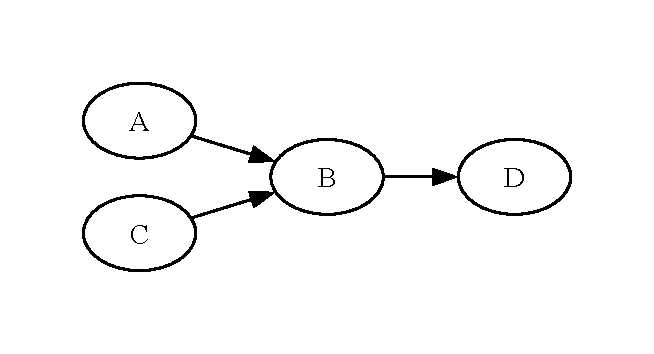
\includegraphics[width=\linewidth]{figs/020-enostavni-graf.pdf}
\end{marginfigure}
%
\vspace*{3mm}
\begin{lstlisting}
import graphviz
from IPython.display import display
dot = graphviz.Digraph()
dot.node('A')
dot.node('B')
dot.edge('A', 'B')
dot.node('C')
dot.edge('C', 'B')
dot.node('D')
dot.edge('B', 'D')
display(dot)
\end{lstlisting}

Koda za izris našega računskega grafa je nekoliko kompleksnejša
(tudi tu sledimo pristopu Andreja Karpathyja). Posebej pomembna je
funkcija \texttt{trace}, ki se rekurzivno sprehodi po grafu, zbere
vozlišča in povezave ter jih topološko uredi. Ta ureditev nam bo
kasneje koristila tudi pri računanju gradientov.

\vspace*{3mm}
\begin{lstlisting}
def trace(root):
    nodes, edges = set(), set()
    def build(v):
        if v not in nodes:
            nodes.add(v)
            for child in v._prev:
                edges.add((child, v))
                build(child)
    build(root)
    return nodes, edges

def draw_dot(root, format='svg', rankdir='LR'):
    """
    format: png | svg | ...
    rankdir: TB (top to bottom graph) | LR (left to right)
    """
    assert rankdir in ['LR', 'TB']
    nodes, edges = trace(root)
    dot = Digraph(format=format, graph_attr={'rankdir': rankdir})
    
    for n in nodes:
        dot.node(name=str(id(n)), label = "{ %s: %.1f }" % \
         (n.label, n.data), shape='record')
        if n._op:
            dot.node(name=str(id(n)) + n._op, label=n._op)
            dot.edge(str(id(n)) + n._op, str(id(n)))
    
    for n1, n2 in edges:
        dot.edge(str(id(n1)), str(id(n2)) + n2._op)
    
    return dot
\end{lstlisting}

Sedaj lahko izrišemo naš računski graf:

\vspace*{3mm}
\begin{lstlisting}
>>> draw_dot(L)
\end{lstlisting}

\begin{figure*}
\includegraphics[width=\linewidth]{figs/020-računski-graf.pdf}
\end{figure*}

Vse je pravilno izračunano. Manjkajo le še odvodi.

\section{Računanje gradientov}

Do tu nam je šlo lepo, a vse, kar smo do sedaj naredili, je bilo računanje vrednosti funkcij. Takih enostavnih, z vsotami in produkti. Manjka nam (vsaj) še izračun gradientov. Te računamo po verižnem pravilu, od zadaj naprej. Torej, od končnih vozlišč s končno vrednostjo funkcije do začetnih vozlišč oziroma vhodnih parametrov. 

Gradiente bomo torej strojno računali tako, da bodo te vozliščem računali njihovi nasledniki, in sicer tako, da jim bodo ustrezno prišteli vrednost lastnega gradienta (vsota) oziroma k tej pomnožili še vrednost sosednega vozlišča (produkt). Vse to bo implementirano v funkciji \texttt{\_backward()}, ki bo lastna vsaki od implementiranih operacij (zaenkrat sta tu le vsota in produkt, kasneje bomo dodali še kakšno drugo funkcijo). Za končni izračun gradienta se moramo sprehoditi po računskemu grafu. To bo storila funkcija \texttt{backward()}, ki se bo najprej topološko uredila vozlišča, potem pa se po njih sprehodila in v vsakem klicala \texttt{\_backward()}.

Še nekaj razmislekov preden razkrijemo zadnjo razširitev naše kode. Gradiente nasledniki prištevajo, ne nastavijo. Na začetku morajo biti gradienti zato postavljeni na vrednosti 0. Prištevanje pa nam koristi v primeru, da ima vozlišče več kot enega naslednika. Npr., v funkciji \( b = a + a \) vsak \( a \) "prinese" po eno 1-ko k odvodu. V nevronskih mrežah, na primer, bodo imela vozlišča računskega grafa tipično veliko naslednikov, in vsak od njih bo k gradientu vozlišča prispeval svojo vrednost. 

Upoštevamo tudi, da je odvod zadnjega vozlišča, torej odvod končne spremenljivke \( L \) po \( L \)-u enak 1. Začnemo torej s to vrednostjo odvoda in jo razširimo od tega, zadnjega vozlišča, nazaj proti začetnim vozliščem. Tu je koda, kjer za vsako od operacij implementiramo funkcijo \texttt{\_backward()}:

\vspace*{3mm}
\begin{lstlisting}
class Value:
    def __init__(self, data, _children=(), _op='', label=''):
        self.data = data
        self.label = label
        self.grad = 0.0
        self._backward = lambda: None
        self._prev = set(_children)
        self._op = _op

    def __repr__(self):
        return f"Value({self.label}: {self.data})"
    
    def __add__(self, other):
        out = Value(self.data + other.data, (self, other), '+')

        def _backward():
            self.grad += 1.0 * out.grad
            other.grad += 1.0 * out.grad
        out._backward = _backward
        return out
    
    def __mul__(self, other):
        out = Value(self.data * other.data, (self, other), '*')

        def _backward():
            self.grad += other.data * out.grad
            other.grad += self.data * out.grad
        out._backward = _backward
        return out
\end{lstlisting}

Manjka le še uporaba funkcij \texttt{\_backward()}. Spomnimo se (morda preveč ponavljamo, a je pomembno), da za dano vozlišče funkcija \texttt{\_backward()} zabeleži vpliv neposrednih predhodnikov danega vozlišča na gradient vozlišča. Če želimo izračunati gradiente za vse spremenljivke v računskem grafu, moram pričeti od zadaj, in v topološkem redu od zadaj naprej za vsako vozlišče pognati \texttt{\_backward()}. Implementacijo takega vzvratnega razširjanja gradientov dodamo v razred \texttt{Value}:

\vspace*{3mm}
\begin{lstlisting}
    def backward(self):
        # topological ordering of the nodes
        topo = []
        visited = set()
        def build_topo(v):
            v.grad = 0
            if v not in visited:
                visited.add(v)
                for child in v._prev:
                    build_topo(child)
                topo.append(v)
        build_topo(self)

        # application of chain rule
        self.grad = 1
        for v in reversed(topo):
            v._backward()
\end{lstlisting}

Preskusimo njeno delovanje na naši enostavni funkciji, torej na tej, za katero smo gradiente računali ročno v prejšnjem poglavju:

\vspace*{3mm}
\begin{lstlisting}
a = Value(2.0, label='a')
b = Value(-3.0, label='b')
c = Value(10.0, label='c')
d = Value(-2.0, label='d')

e = a * b
e.label = 'e'
f = e + c
f.label = 'f'
L = f * d
L.label = 'L'

L.backward()
\end{lstlisting}

Izpišimo še vrednosti gradientov:

\vspace*{3mm}
\begin{lstlisting}
>>> a.grad, b.grad, c.grad, d.grad
(6.0, -4.0, -2.0, 4.0)
\end{lstlisting}

Juhu! Dela. Oziroma, bolje rečeno, pravilno izračuna vrednosti gradientov za našo enostavno funkcijo. Enostavno zato, ker ta samo sešteva in množi. Spodaj je še izris računskega grafa z odvodi:

\begin{figure*}
\includegraphics[width=\linewidth]{figs/020-računski-graf-odvodi.pdf}
\end{figure*}

\section{Konstante, negacija, potenciranje}

Pri malce bolj kompleksnih funkcijah bi želeli v naših računskih grafih obravnavati tudi konstate, računali razlike, potence... Oziroma, delali z izrazi, kot so na primer spodnji:

\vspace*{3mm}
\begin{lstlisting}
>>> a = Value(3, 'a')
>>> b = Value(42, 'b')
>>> a + 10
>>> -13 + a
>>> a - b
>>> (a + b) ** 3
\end{lstlisting}

Pri vseh teh nam naša trenutna implementacija vrne napako. Potrebno jo bo zato razširiti. Za operacije s konstantami bomo avtomatsko dodali novo vozlišče, za to, da bodo te lahko v naših operacijah tudi na levi strani, bomo implementirali funkcije, kot je \texttt{\_\_radd\_\_}, odštevanje bomo implementirali s seštevanje z negativno vrednostjo desnega operanda, spisali pa bomo tudi novo operacijo za potenciranje. Spodaj je tako razširjena implementacija razreda \texttt{Value}:

\vspace*{3mm}
\begin{lstlisting}
class Value:
    def __init__(self, data, _children=(), _op='', label=''):
        self.data = data
        self.label = label
        self.grad = 0.0
        self._backward = lambda: None
        self._prev = set(_children)
        self._op = _op

    def __repr__(self):
        return f"Value({self.label}: {self.data})"
    
    def __add__(self, other):
        other = other if isinstance(other, Value) else Value(other)
        out = Value(self.data + other.data, (self, other), '+')

        def _backward():
            self.grad += out.grad
            other.grad += out.grad
        out._backward = _backward

        return out
    
    def __mul__(self, other):
        other = other if isinstance(other, Value) else Value(other)
        out = Value(self.data * other.data, (self, other), '*')

        def _backward():
            self.grad += other.data * out.grad
            other.grad += self.data * out.grad
        out._backward = _backward
        return out
    
    def __pow__(self, other):
        out = Value(self.data ** other, (self, ), f'**{other}')

        def _backward():
            self.grad += other * (self.data ** (other - 1)) * out.grad
        out._backward = _backward
        return out
    
    def __radd__(self, other):  # other + self
        return self + other
    
    def __neg__(self): # - self
        return self * -1
    
    def __sub__(self, other):
        return self + (-other)
    
    def __rsub__(self, other):  # other - self
        return other + (-self)

    def __rmul__(self, other):  # other * self
        return self * other
\end{lstlisting}

Iz zgornjega zapisa smo izpustili funkcijo \texttt{backward()}, ki ostane enaka kot prej. S kodo, kot jo imamo spisano zgoraj, lahko sedaj implementirano gradientni sestop za funkcijo iz prejšnjega poglavja:

\vspace*{3mm}
\begin{lstlisting}
a = Value(0, label='a')
for _ in range(50):
    L = a**2 - 10 * a + 28
    backward(L)
    a.data -= 0.1 * a.grad
    print(L.data, a.data)
\end{lstlisting}

Tu je čas za bralca, da preskusi delovanje naše kode, jo morda preoblikuje v knjižnico in doda izračun in odvajanje za še kakšne dodatne funkcije. Mi pa se bomo spustili v nove podvige v naslednjem poglavju, ko bomo to kodo za avtomatsko odvajanje uporabili na bolj resnih primerih, kjer bodo (kriterijske) funkcije uporabljale tudi zunanje podatke in na primer tako implementirale iskanje modela za linearno regresijo ali njeno regularizirano inačico. Z zgornjimi, in morda še kakšnimi drugi manjšimi razširitvami, smo sedaj torej pripravljeni za ``resno'' uporabo naše male knjižnice za avtomatsko odvajanje.